\chapter{Logarithms}

After the world had created exponents, it needed the opposite. We
could talk about the quantity $? = 2^3$, that is, ``What is the
product of 2 multiplied by itself three times?''  We needed some way
to talk about $2^? = 8$, that is ``2 to the what is 8?'' So we
developed the logarithm.\index{logarithm} \index{log}

Here is an example:

$$\log_{2}8 = 3$$

In English, you would say ``The logarithm base 2 of 8 is 3.''

The base (2, in this case) can be any positive number. The argument
(8, in this case) can also be any positive number.

Try this one: What is the logarithm base 2 of 1/16?

You know that $2^{-4} = \frac{1}{16}$, so $\log_{2} \frac{1}{16} = -4$.

\section{Logarithms in Python}

Most calculators have pretty limited logarithm capabilities, but
python has a nice \pyfunction{log} function that lets you specify both
the argument and the base.  Start python, import the math module, and try taking a few logarithms:\index{log!in python}

\begin{Verbatim}
>>> import math
>>> math.log(8,2)
3.0
>>> math.log(1/16, 2)
-4.0
\end{Verbatim}

Let's say that a friend offers you 5\% interest per year on your
investment for as long as you want. And you wonder, ``How many years
before my investment is 100 times as large?'' You can solve this problem with logarithms:

\begin{Verbatim}
>>> math.log(100, 1.05)
94.3872656381287
\end{Verbatim}

If you leave your investment with your friend for 94.4 years, the
investment will be worth 100 times what you put in.

\section{Logarithm Identities}

The logarithm is defined this way:\index{logarithm!identities}

$$\log_b a = c \iff b^c = a$$

Notice that the logarithm of 1 is always zero, and $\log_b b = 1$.

The logarithm of a product:

$$\log_b a c = \log_b a + \log_b c$$

This follows from the fact that $b^{a + c} = b^a b^c$. What about a quotient?

$$\log_b \frac{a}{c} = \log_b a - \log_b c$$

Exponents?

$$\log_b \left(a^c\right) = c \log_b a$$

Notice that because logs and exponents are the opposite of each other, they can cancel each other out:

$$b^{\log_b a} = a$$

and

$$\log_b \left(b^a\right) = a$$

\section{Changing Bases}

I mentioned that most calculators have pretty limited logarithm
capabilities. Most calculators don't allow you to specify what base
you want to work with. All scientific calculators have a button for
``log base 10''.  So you need to know how to use that button to get
logarithms for other bases. Here is the change-of-base identity:\index{logarithm!change of base}

$$\log_b a = \frac {\log_c a}{\log_c b}$$

So, for example, if you wanted to find $\log_2 8$, you would ask the
calculator for $\log_{10} 8$ and then divide that by $\log_{10} 2$.
You should get 3.

\section{Natural Logarithm}

When you learn about circles, you are told that the circumference of a
circle is about 3.141592653589793 times its diameter.  Because we use
this unweildy number a lot, we give it a name: We say ``The
circumference of a circle is $\pi$ times its diameter.''

There is a second unweildy number that we will eventually use a lot in
solving problems.  It is about 2.718281828459045 (but the digits
actually go on forever, just like $\pi$). We call this number $e$. (I'm
not going to tell you why $e$ is special now, but soon...)\index{e}\index{logarithm!natural}

Most calculators have a button labeled ``ln''.  That is the
\textit{natural logarithm} button. It takes the log in base $e$.\index{ln}

Similarly, in python, if you don't specify a base, the logarithm is done in base $e$:

\begin{Verbatim}
>>> math.log(10)
2.302585092994046
>>> math.log(math.e)
1.0
\end{Verbatim}

\section{Logarithms in Spreadsheets}

Spreadsheets have three log functions:
\begin{itemize}
\item \pyfunction{LOG} takes both the argument and the base. \pyfunction{LOG(8,2)} returns 3.
\item \pyfunction{LOG10} takes just the argument and uses 10 as the base.
\item \pyfunction{LN} takes just the argument and uses $e$ as the base.
\end{itemize}

Here is a plot from a spreadsheet of a graph of $y = LOG(x, 2)$.

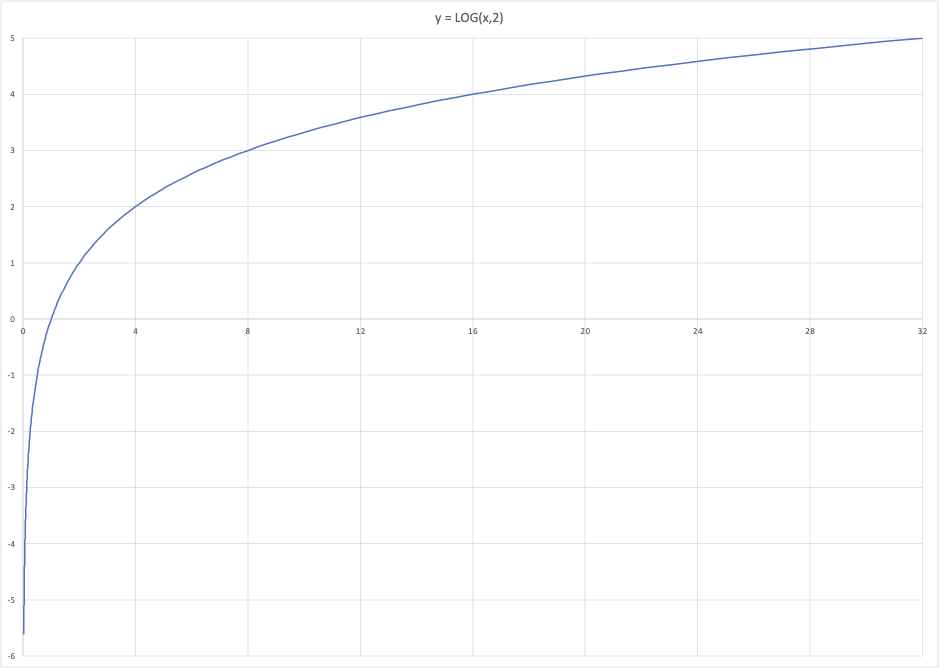
\includegraphics[width=0.8\textwidth]{log_graph.png}

Spreadsheets also have the function \pyfunction{EXP(x)} which returns
$e^x$.  For example, \pyfunction{EXP(2)} returns 7.38905609893065.

